\documentclass[portrait,final,a0paper,fontscale=0.277]{baposter}

\usepackage{calc}
\usepackage{graphicx}
\usepackage{amsmath}
\usepackage{amssymb}
\usepackage{relsize}
\usepackage{multirow}
\usepackage{rotating}
\usepackage{bm}
\usepackage{enumitem}
\usepackage{url}
\usepackage{booktabs}

\usepackage{graphicx}
\usepackage{multicol}

%\usepackage{times}
%\usepackage{helvet}
%\usepackage{bookman}
\usepackage{palatino}

\newcommand{\captionfont}{\footnotesize}

\graphicspath{{images/}{../images/}}
\usetikzlibrary{calc}


\newcommand{\Matrix}[1]{\begin{bmatrix} #1 \end{bmatrix}}
\newcommand{\Vector}[1]{\begin{pmatrix} #1 \end{pmatrix}}

\newcommand*{\norm}[1]{\mathopen\| #1 \mathclose\|}% use instead of $\|x\|$
\newcommand*{\abs}[1]{\mathopen| #1 \mathclose|}% use instead of $\|x\|$
\newcommand*{\normLR}[1]{\left\| #1 \right\|}% use instead of $\|x\|$

\newcommand*{\SET}[1]  {\ensuremath{\mathcal{#1}}}
\newcommand*{\FUN}[1]  {\ensuremath{\mathcal{#1}}}
\newcommand*{\MAT}[1]  {\ensuremath{\boldsymbol{#1}}}
\newcommand*{\VEC}[1]  {\ensuremath{\boldsymbol{#1}}}
\newcommand*{\CONST}[1]{\ensuremath{\mathit{#1}}}

\DeclareMathOperator*{\argmax}{arg\,max}
\DeclareMathOperator*{\diag}{diag}
\DeclareMathOperator*{\argmin}{arg\,min}
\DeclareMathOperator*{\vectorize}{vec}
\DeclareMathOperator*{\reshape}{reshape}

%\font\dsfnt=dsrom12

\newcommand{\SNN}{\ensuremath{\mathbb N}}
\newcommand{\SRR}{\ensuremath{\mathbb R}}
\newcommand{\SZZ}{\ensuremath{\mathbb Z}}
%-----------------------------------------------------------------------------
% Matrices of the shape model
\renewcommand{\a}{\VEC\alpha}
\renewcommand{\v}{\VEC v}
\renewcommand{\l}{\VEC l}
\newcommand*{\m}{\VEC{\mu}}
\newcommand*{\M}{\MAT{M}}
\renewcommand*{\P}{\MAT{\Pi}}

%\newcommand{\J}{\SET J}
\newcommand{\J}{\SET{P}}
\newcommand{\Active}{\mathcal{A}}
\newcommand{\Selection}{\mathbf{S}}
\newcommand{\AllSelections}{\mathfrak{S}}
\newcommand{\Params}{\VEC\Theta}

%%%%%%%%%%%%%%%%%%%%%%%%%%%%%%%%%%%%%%%%%%%%%%%%%%%%%%%%%%%%%%%%%%%%%%%%%%%%%%%%
%%%% Some math symbols used in the text
%%%%%%%%%%%%%%%%%%%%%%%%%%%%%%%%%%%%%%%%%%%%%%%%%%%%%%%%%%%%%%%%%%%%%%%%%%%%%%%%

%%%%%%%%%%%%%%%%%%%%%%%%%%%%%%%%%%%%%%%%%%%%%%%%%%%%%%%%%%%%%%%%%%%%%%%%%%%%%%%%
% Multicol Settings
%%%%%%%%%%%%%%%%%%%%%%%%%%%%%%%%%%%%%%%%%%%%%%%%%%%%%%%%%%%%%%%%%%%%%%%%%%%%%%%%
\setlength{\columnsep}{1.5em}
\setlength{\columnseprule}{0mm}

%%%%%%%%%%%%%%%%%%%%%%%%%%%%%%%%%%%%%%%%%%%%%%%%%%%%%%%%%%%%%%%%%%%%%%%%%%%%%%%%
% Save space in lists. Use this after the opening of the list
%%%%%%%%%%%%%%%%%%%%%%%%%%%%%%%%%%%%%%%%%%%%%%%%%%%%%%%%%%%%%%%%%%%%%%%%%%%%%%%%
\newcommand{\compresslist}{%
\setlength{\itemsep}{1pt}%
\setlength{\parskip}{0pt}%
\setlength{\parsep}{0pt}%
}

%%%%%%%%%%%%%%%%%%%%%%%%%%%%%%%%%%%%%%%%%%%%%%%%%%%%%%%%%%%%%%%%%%%%%%%%%%%%%%
%%% Begin of Document
%%%%%%%%%%%%%%%%%%%%%%%%%%%%%%%%%%%%%%%%%%%%%%%%%%%%%%%%%%%%%%%%%%%%%%%%%%%%%%

\begin{document}

%%%%%%%%%%%%%%%%%%%%%%%%%%%%%%%%%%%%%%%%%%%%%%%%%%%%%%%%%%%%%%%%%%%%%%%%%%%%%%
%%% Here starts the poster
%%%---------------------------------------------------------------------------
%%% Format it to your taste with the options
%%%%%%%%%%%%%%%%%%%%%%%%%%%%%%%%%%%%%%%%%%%%%%%%%%%%%%%%%%%%%%%%%%%%%%%%%%%%%%
% Define some colors

\definecolor{JINGTAILAN}{HTML}{2775b6}
\definecolor{YUEBAI}{HTML}{eef7f2}
\definecolor{QINGSHUILAN}{HTML}{93d5dc}

\hyphenation{resolution occlusions}
%%
\begin{poster}%
  % Poster Options
  {
  % Show grid to help with alignment
  grid=false,
  columns=6,
  % Column spacing
  colspacing=1em,
  % Color style
  bgColorOne=YUEBAI,
  bgColorTwo=white,
  borderColor=QINGSHUILAN,
  %headerColorOne=QINGSHUILAN,
  %headerColorTwo=QINGSHUILAN,,
  headerFontColor=JINGTAILAN,
  boxColorOne=YUEBAI,
  boxColorTwo=JINGTAILAN,
  % Format of textbox
  textborder=faded,
  % Format of text header
  eyecatcher=true,
  headerborder=closed,
  headerheight=0.1\textheight,
%  textfont=\sc, An example of changing the text font
  headershape=roundedright,
  headershade=shadelr,
  headerfont=\Large\bf\textsc, %Sans Serif
  textfont={\setlength{\parindent}{1.5em}},
  boxshade=plain,
%  background=shade-tb,
  background=plain,
  linewidth=2pt
  }
  % Eye Catcher
  {
  %\includegraphics[height=7em]{images/search_tree_ex1-crop.pdf}
  } 
  % Title
  {\bf\textsc{Recherche comparative du modèle de coût pour la normalisation et la dénormalisation de BD NoSQL}\vspace{0.5em}}
  % Authors
  {\textsc{Réalisé par : Hao ZHANG \ \ \ \ \ \ \ Encadré par : Nicolas TRAVERS}}
  % University logo
  {% The makebox allows the title to flow into the logo, this is a hack because of the L shaped logo.
    \includegraphics[height=9.0em]{logos/logo_esilv.png}
  }

%%%%%%%%%%%%%%%%%%%%%%%%%%%%%%%%%%%%%%%%%%%%%%%%%%%%%%%%%%%%%%%%%%%%%%%%%%%%%%
%%% Now define the boxes that make up the poster
%%%---------------------------------------------------------------------------
%%% Each box has a name and can be placed absolutely or relatively.
%%% The only inconvenience is that you can only specify a relative position 
%%% towards an already declared box. So if you have a box attached to the 
%%% bottom, one to the top and a third one which should be in between, you 
%%% have to specify the top and bottom boxes before you specify the middle 
%%% box.
%%%%%%%%%%%%%%%%%%%%%%%%%%%%%%%%%%%%%%%%%%%%%%%%%%%%%%%%%%%%%%%%%%%%%%%%%%%%%%
    %
    % A coloured circle useful as a bullet with an adjustably strong filling
    \newcommand{\colouredcircle}{%
      \tikz{\useasboundingbox (-0.2em,-0.32em) rectangle(0.2em,0.32em); \draw[draw=black,fill=lightblue,line width=0.03em] (0,0) circle(0.18em);}}

%%%%%%%%%%%%%%%%%%%%%%%%%%%%%%%%%%%%%%%%%%%%%%%%%%%%%%%%%%%%%%%%%%%%%%%%%%%%%%
  \headerbox{Contexte}{name=contexte,column=0,span=2,row=0}{
%%%%%%%%%%%%%%%%%%%%%%%%%%%%%%%%%%%%%%%%%%%%%%%%%%%%%%%%%%%%%%%%%%%%%%%%%%%%%%
Dans le BigData, les bases NoSQL répondent au problème de stockage et de      distribution des données à large échelle pour souvent répondre à des problèmes de performances en centralisé.
  
De nombreuses solutions existent, et faire le bon choix lors de la définition des besoins d'un Système d'Information devient un choix crucial, car il est difficile et risqué de faire un changement technologique.
 }

%%%%%%%%%%%%%%%%%%%%%%%%%%%%%%%%%%%%%%%%%%%%%%%%%%%%%%%%%%%%%%%%%%%%%%%%%%%%%%
  \headerbox{Objectif}{name=objectif,column=2,span=2,row=0}{
%%%%%%%%%%%%%%%%%%%%%%%%%%%%%%%%%%%%%%%%%%%%%%%%%%%%%%%%%%%%%%%%%%%%%%%%%%%%%%
Le but de ce projet de recherche est de définir un modèle de coût d'évaluation de requêtes sur des solutions NoSQL.

Ainsi, ce modèle de coût (accès réseaux et accès locaux) sera capable d'estimer pour chaque type de requête ce qu'il en coûtera, et ainsi de choisir la solution NoSQL qui minimise ce coût.

L'objectif de ce projet est donc de raffiner les modèles de coût existant dans la littérature pour avoir un modèle plus global, le plus précis possible. 
  }

%%%%%%%%%%%%%%%%%%%%%%%%%%%%%%%%%%%%%%%%%%%%%%%%%%%%%%%%%%%%%%%%%%%%%%%%%%%%%%
\headerbox{Bases des données du test}{name=BD_text,column=4,span=2,row=0}{
  %%%%%%%%%%%%%%%%%%%%%%%%%%%%%%%%%%%%%%%%%%%%%%%%%%%%%%%%%%%%%%%%%%%%%%%%%%%%%%
\centering{{\includegraphics[width=0.95\linewidth]{pics/environnement.png}}}\\[0em]%
\centering{Schéma des collections des bases de données}\\[0em]%

\centering{{\includegraphics[width=0.8\linewidth]{pics/modelisation.png}}}\\[0em]%
\centering{Modélisation de semi-dénormalisation et dénormalisation}\\[0em]%
}
%%%%%%%%%%%%%%%%%%%%%%%%%%%%%%%%%%%%%%%%%%%%%%%%%%%%%%%%%%%%%%%%%%%%%%%%%%%%%%
  \headerbox{Résultats}{name=representation,column=3,span=3,below=BD_text}{
%%%%%%%%%%%%%%%%%%%%%%%%%%%%%%%%%%%%%%%%%%%%%%%%%%%%%%%%%%%%%%%%%%%%%%%%%%%%%%
\centering\includegraphics[width=0.825\linewidth]{pics/1.png}\\[0em]
\centering{Résultats de temps moyen avec l'écart type}\\[0em]%
\centering\includegraphics[width=0.825\linewidth]{pics/2.png}\\[0em]
\centering{Résultats des tests par chaque fois de test}\\[0em]%
  }
%%%%%%%%%%%%%%%%%%%%%%%%%%%%%%%%%%%%%%%%%%%%%%%%%%%%%%%%%%%%%%%%%%%%%%%%%%%%%%
  \headerbox{Techniques}{name=techniques,column=0,span=2,below=contexte}{
%%%%%%%%%%%%%%%%%%%%%%%%%%%%%%%%%%%%%%%%%%%%%%%%%%%%%%%%%%%%%%%%%%%%%%%%%%%%%%
\centering{{\includegraphics[width=0.85\linewidth]{pics/mongo_python.png}}}\\[0em]%
\centering{MongoDB, Python et PyMongo}\\[0em]%
  }
%%%%%%%%%%%%%%%%%%%%%%%%%%%%%%%%%%%%%%%%%%%%%%%%%%%%%%%%%%%%%%%%%%%%%%%%%%%%%%
  \headerbox{Source Code}{name=source,column=2,span=2,below=objectif}{
  \centering{{\includegraphics[width=0.25\linewidth]{pics/QR.png}}}\\[0em]%
%%%%%%%%%%%%%%%%%%%%%%%%%%%%%%%%%%%%%%%%%%%%%%%%%%%%%%%%%%%%%%%%%%%%%%%%%%%%%%
  %\noindent
  %\begin{minipage}{\linewidth}
  %\begin{minipage}{0.75\linewidth}
    %\indent{}The source code is available at \\
    %\url{http://www.cs.unibas.ch/personen/amberg_brian/bnb/}
  %\end{minipage}\hfill%
  %\begin{minipage}{0.23\linewidth}
  %\hfill\includegraphics[width=\linewidth]{chart}
  %\end{minipage}
  %\end{minipage}
  }
%%%%%%%%%%%%%%%%%%%%%%%%%%%%%%%%%%%%%%%%%%%%%%%%%%%%%%%%%%%%%%%%%%%%%%%%%%%%%%
  \headerbox{État de l'art}{name=etat_de_l_art,column=0,below=techniques,column=0,span=3}{
%%%%%%%%%%%%%%%%%%%%%%%%%%%%%%%%%%%%%%%%%%%%%%%%%%%%%%%%%%%%%%%%%%%%%%%%%%%%%%
\centering{{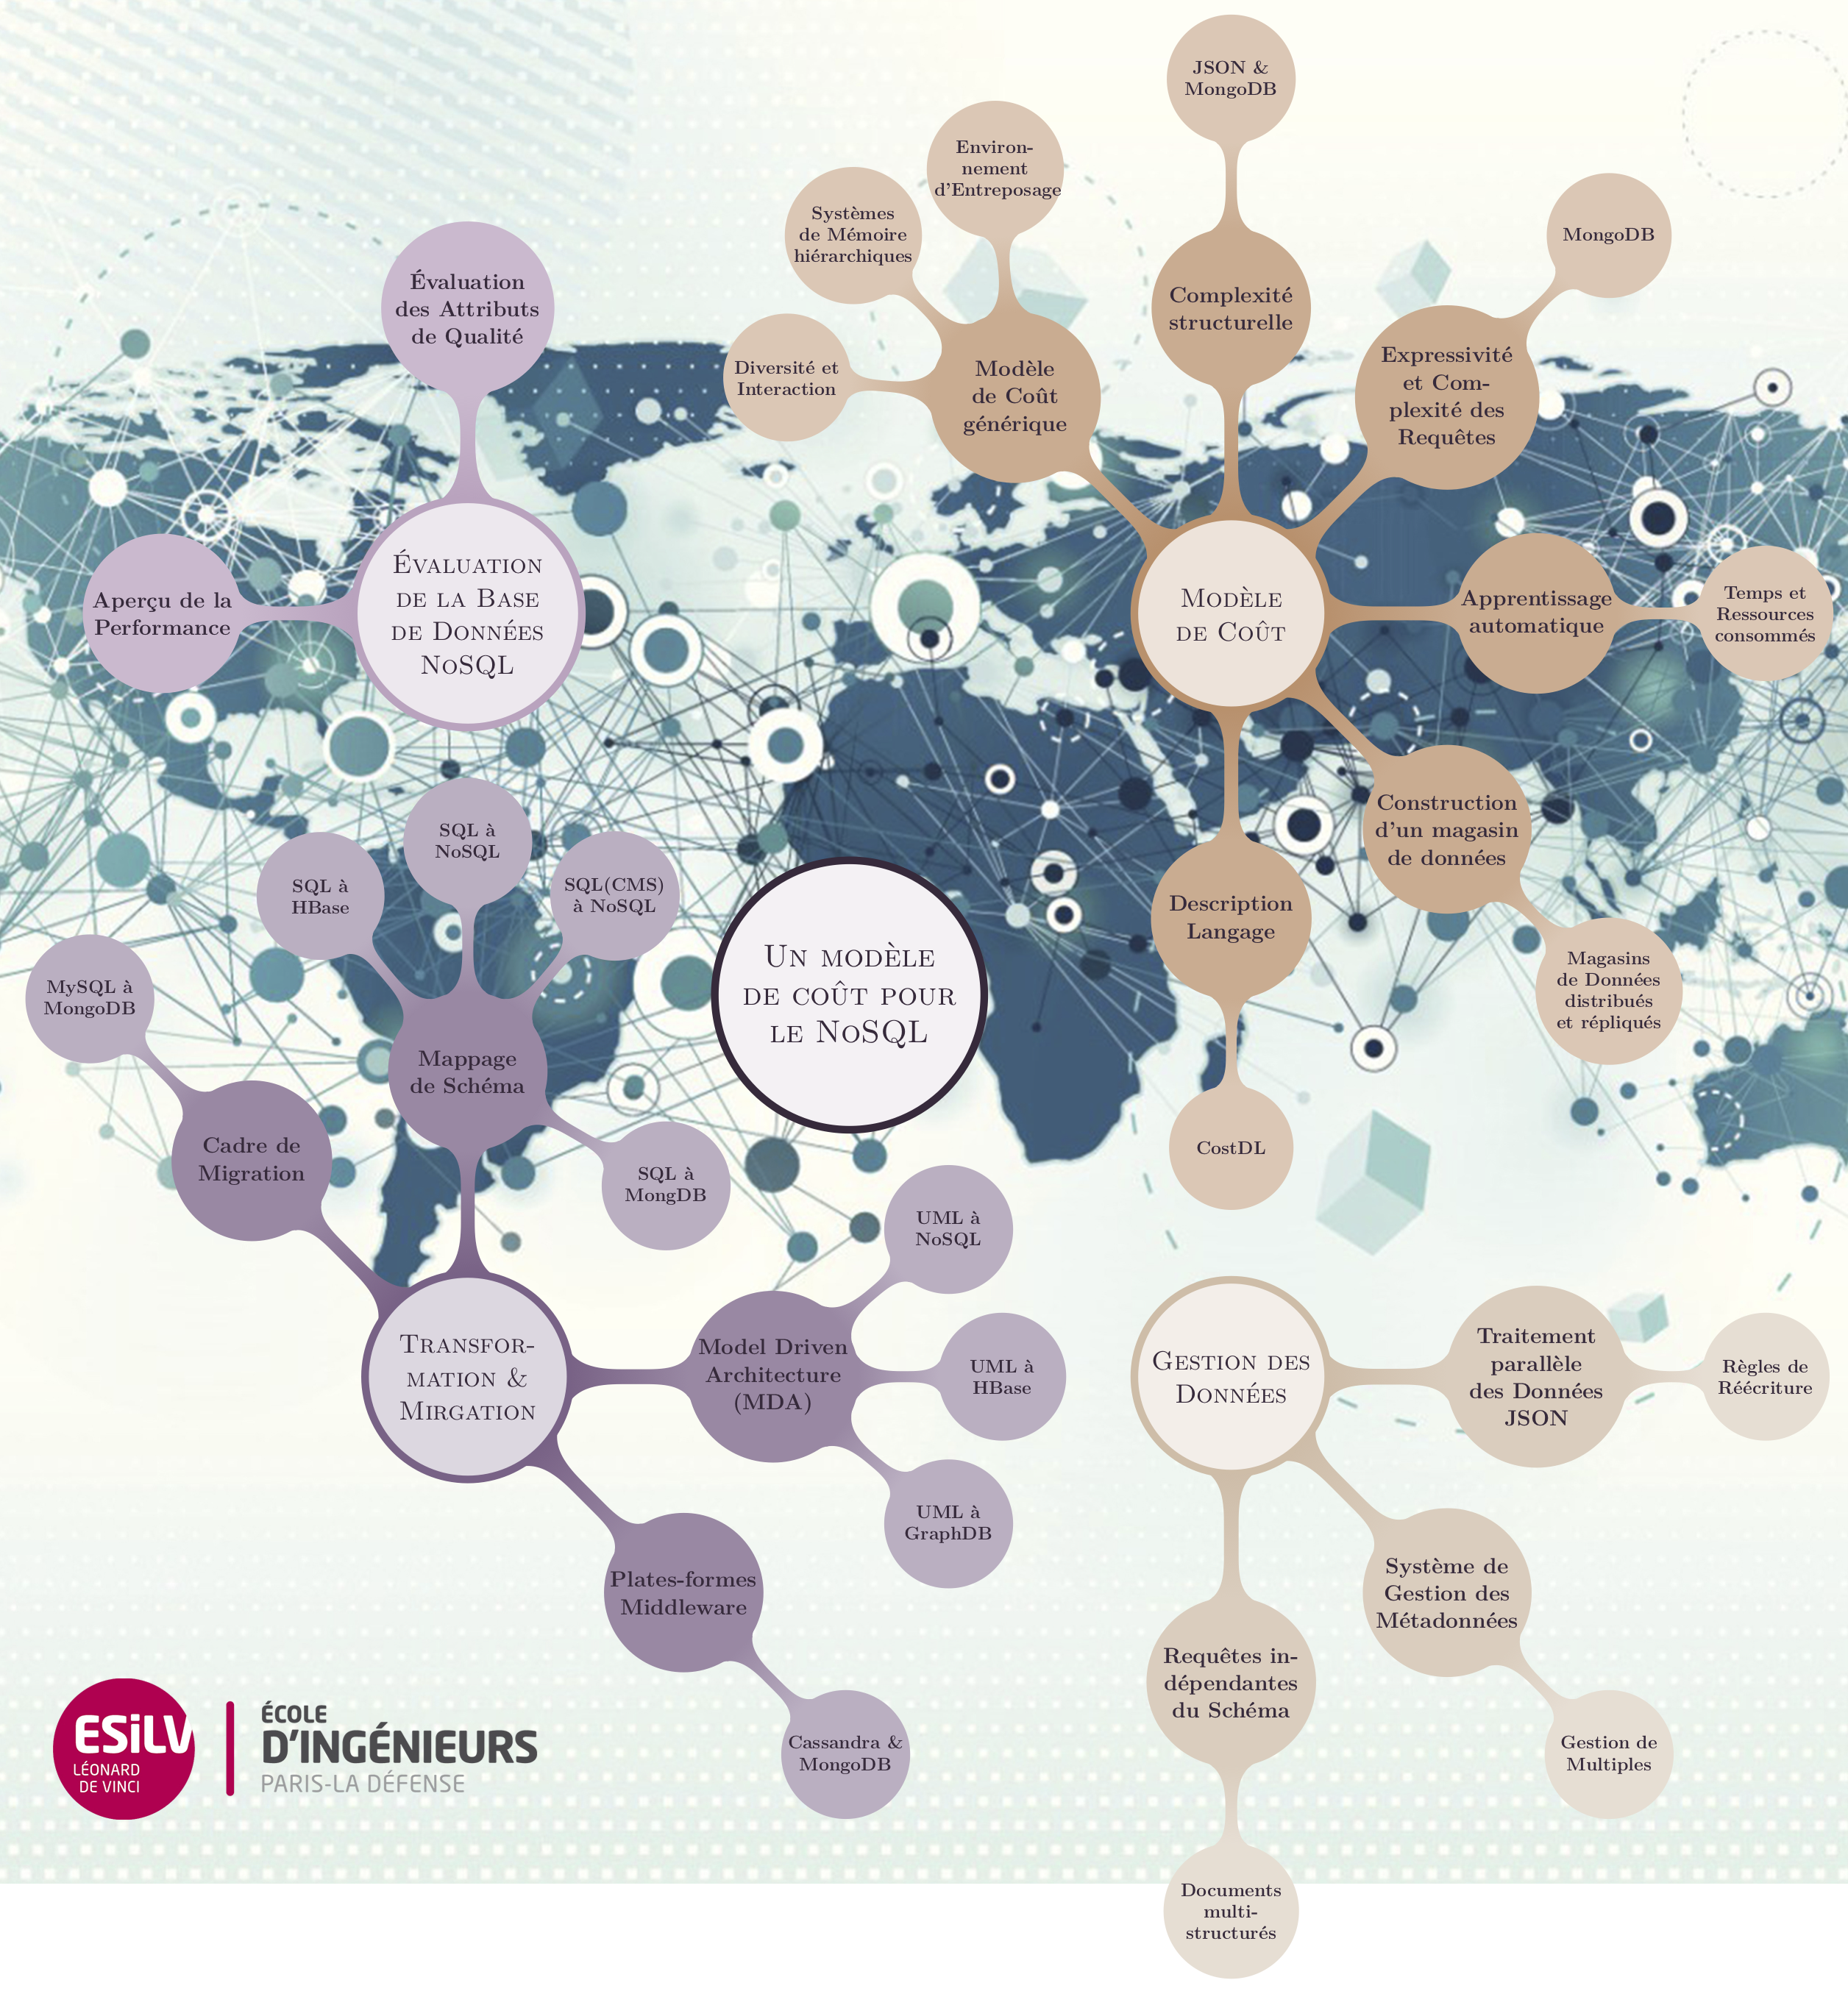
\includegraphics[width=0.85\linewidth]{pics/mindmap.png}}}\\[0em]%
\centering{Classification des articles scientifiques}\\[0em]%
\begin{enumerate}
 \item Évaluation de la Base de Données NoSQL
 \item Transformation et Mirgation vers NoSQL
 \item Modèle de coût d'une base de données
 \item Gestion de la  base de données NoSQL
 \end{enumerate}
}

%%%%%%%%%%%%%%%%%%%%%%%%%%%%%%%%%%%%%%%%%%%%%%%%%%%%%%%%%%%%%%%%%%%%%%%%%%%%%%
\headerbox{Requêtes}{name=requetes,column=0,span=3,above=bottom}{
  %%%%%%%%%%%%%%%%%%%%%%%%%%%%%%%%%%%%%%%%%%%%%%%%%%%%%%%%%%%%%%%%%%%%%%%%%%%%%%
\begin{enumerate}
 \item[C] Create : créer une nouvelle commande avec 10 articles différents
 \item[R] Read : chercher aléatoirement l'information d'un client par son nom et prénom en montrant l'id de la plus nouvelle commande
 \item[U] Update : modifier le temps de livraison des dix articles les plus anciens qui ne sont pas encore délivrés
 \item[D] Delete : supprimer aléatoirement d'une commande pas encore livrée
 \end{enumerate}
  }

\end{poster}

\end{document}

